
This thesis addresses that OLAP over large property graph is important but current graph databases process graph OLAP in an overwelmingly inefficient manner, and provides an end-to-end efficient solution for it.

%----------------------------------------------------------------------
\section{Property Graph Model}
%----------------------------------------------------------------------

We are living in an age with exponential growth of data, and a world that is more and more connected. When a user creates a new post not only a post is created,  a “creates” connection between the user and the post is established as well. When the user tags the post with a tag, a “has tag” connection is built between the tag and the post. When a bank transfer happens, a “transfers” connection between two accounts is created. With the fast development of Web2.0 and Internet of Things(IoT), numerous connections of various kinds are created every second. As a result, massive amount of data of connected systems is generated at the same time. 

Property graph is a widely used model for connected systems. A property graph is made of nodes, edges, and properties. Like general graph data models, nodes represent entities and edges represent relationships. For instance, below is a property graph of an online Q\&A forum named www.StackExchange.com. It shows the connections of users (represented by red nodes) and posts( represented by blue nodes). Each arrow from a user node and to a post node represents a “creates” connection. We can view “user creates post” connections clearly from the graph.


\begin {figure}[H]
\centering
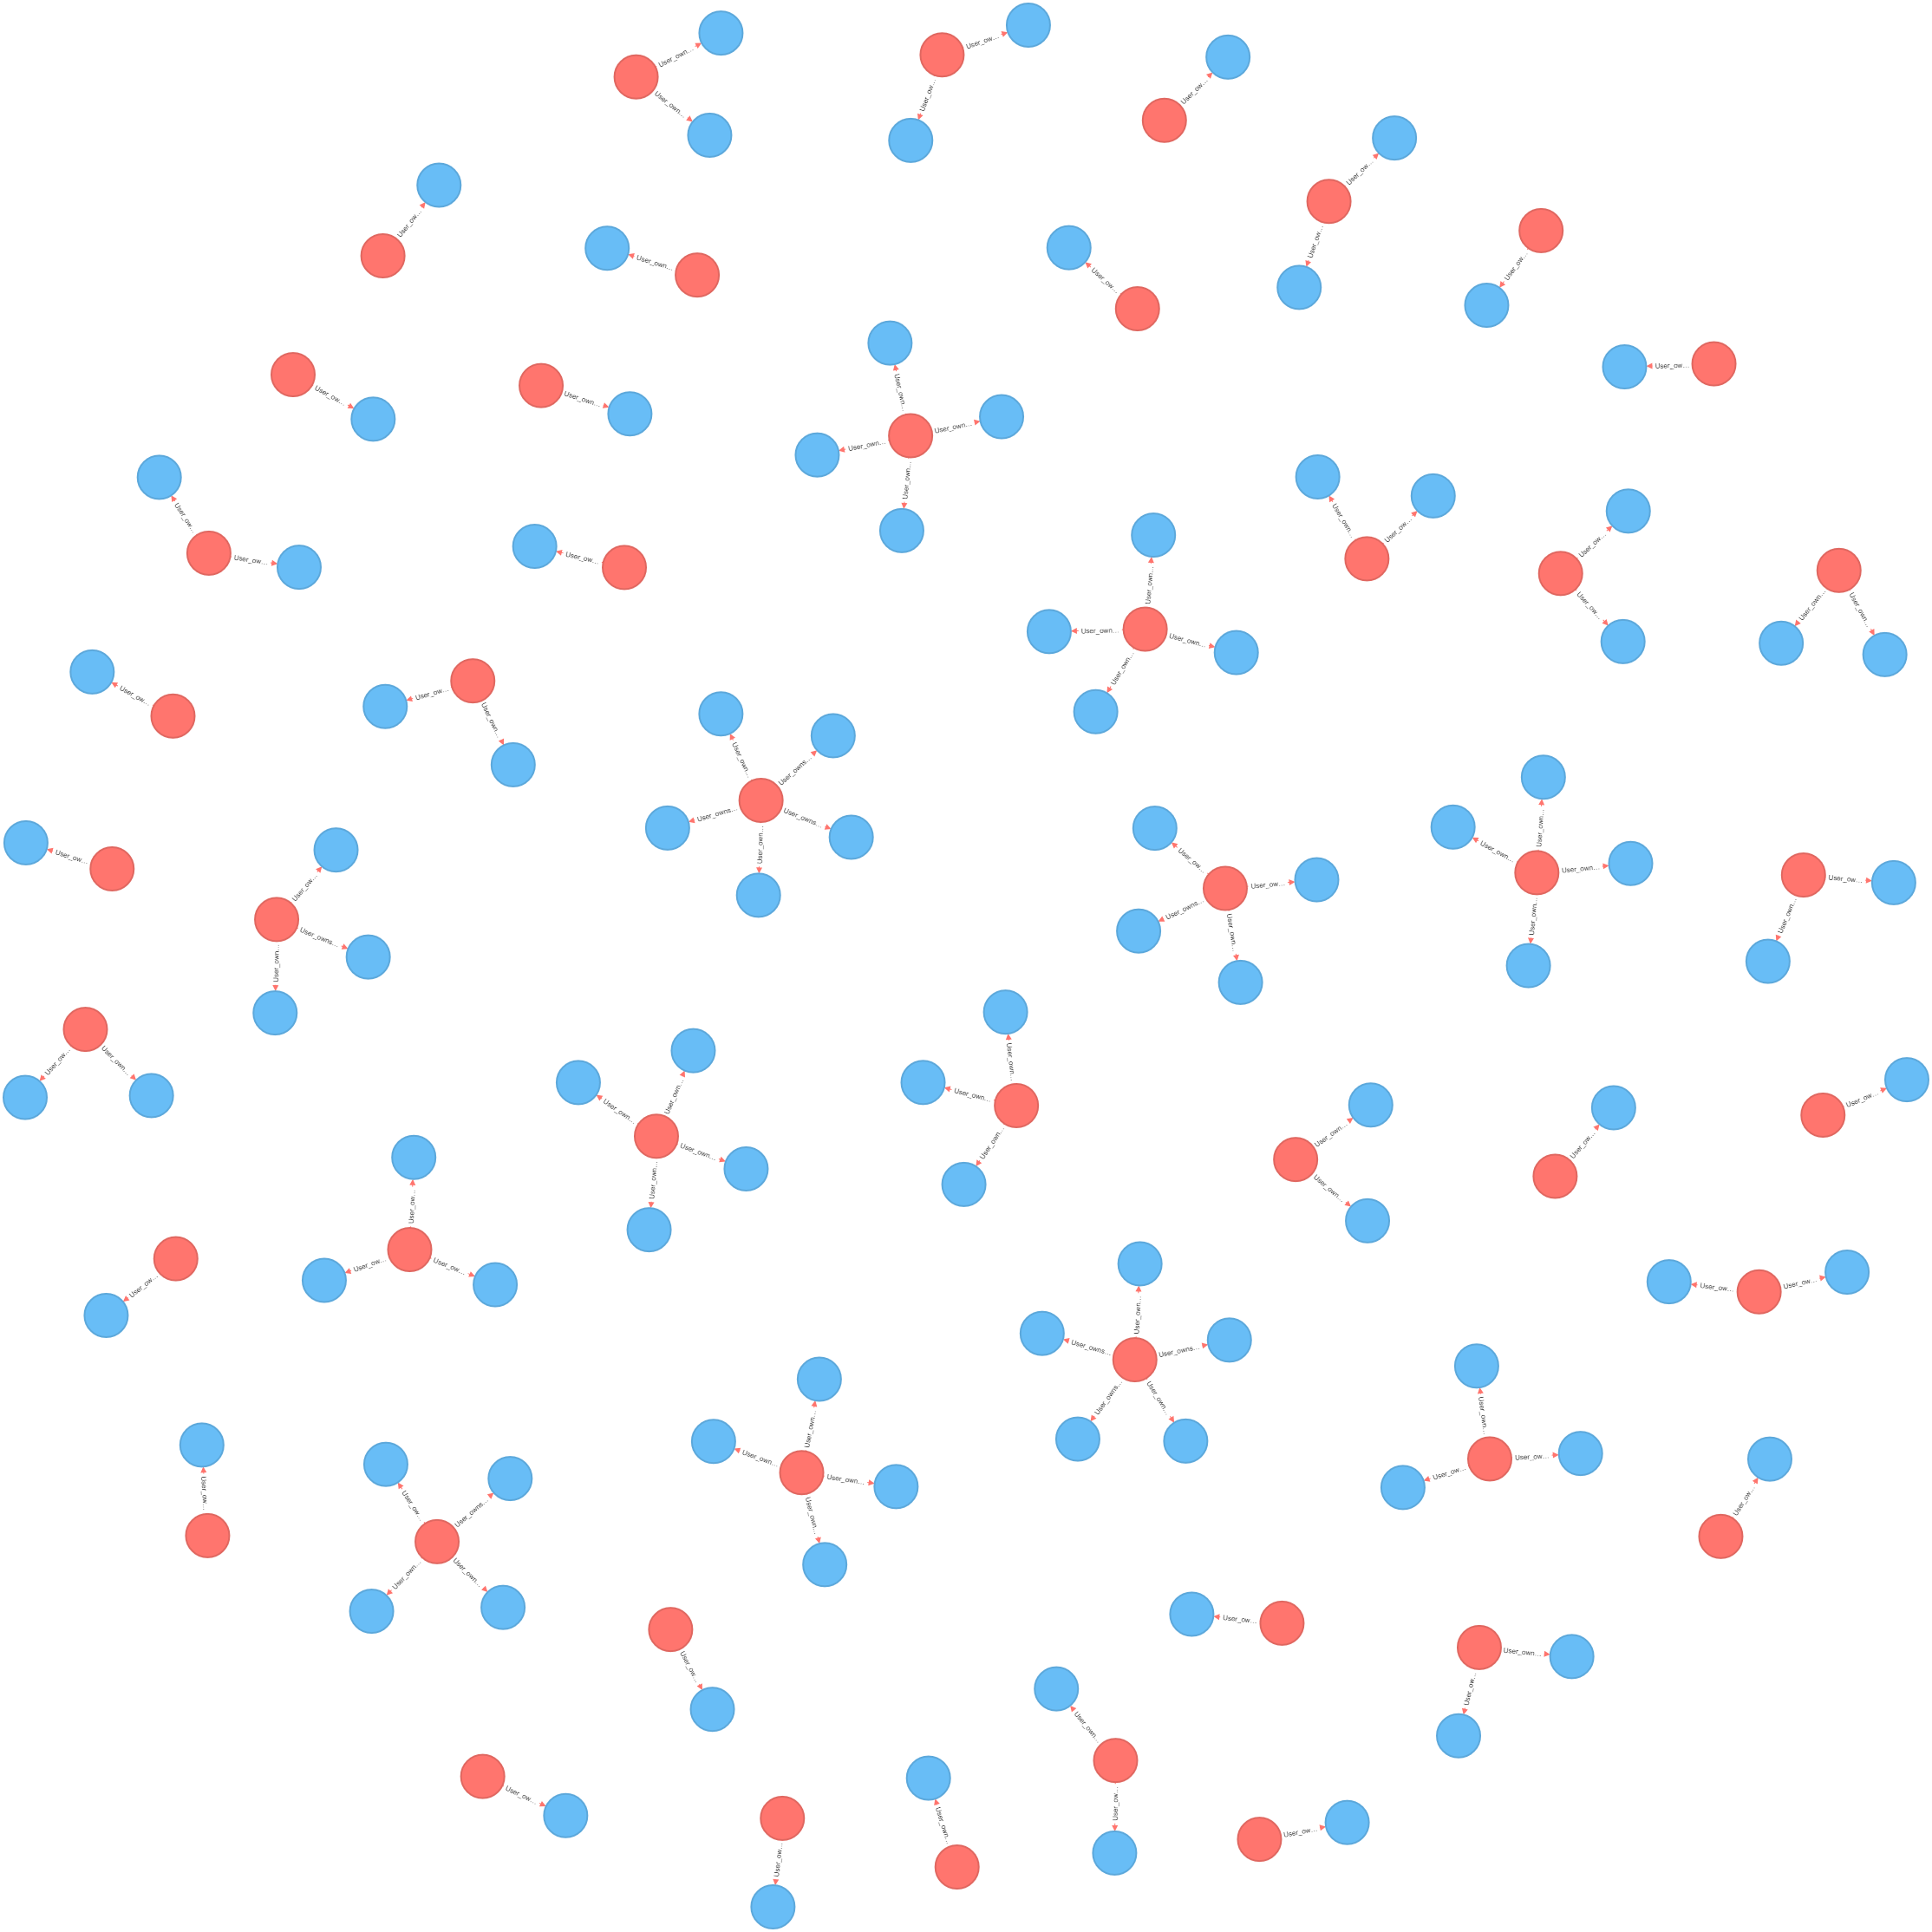
\includegraphics[scale=0.07]{pic/1.png}
\end{figure}


Besides nodes and edges, in property graph nodes and edges can have any number and type of properties. 


\begin {figure}[H]
\centering
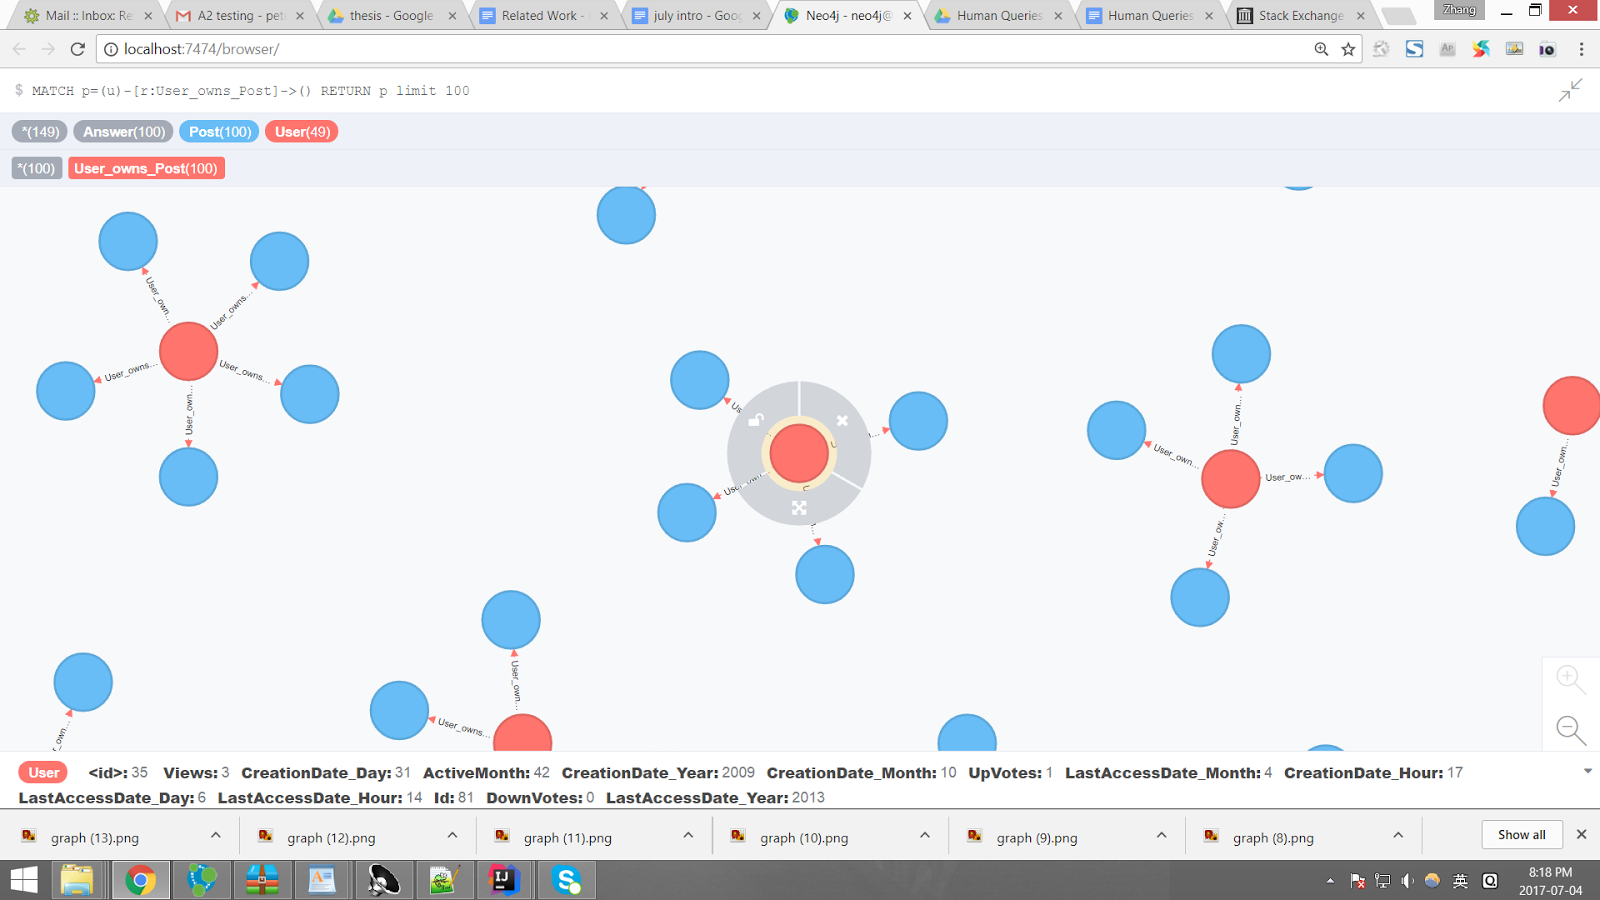
\includegraphics[scale=0.2]{pic/2.png}
\end{figure}

For instance, in the exampling property graph, the highlighted User node has properties like the user’s Age, Views, UpVotes etc(listed at the end of the picture). Notice that there is no restriction on what properties a User node can have . That is, any node or edge could be freely attributed with any type of property. This makes a property graph very flexible in terms of property attribution.
 
Property graph is an informative model as it contains not only nodes and edges, but properties of each individual node and edge as well. Let’s look at a property graph of www.stackexchange.com with contains:

Nodes:	User(in red).
Post(in blue). 
Tag(in green). 
 
Edges: 		User\_owns\_Post(in red). 
Post\_hastag\_Tag(in blue).
 
Properties:	User’s View, Post’s Score, Tag’s Tagname ect.
 
A snapshot of data graph: 

\begin {figure}[H]
\centering
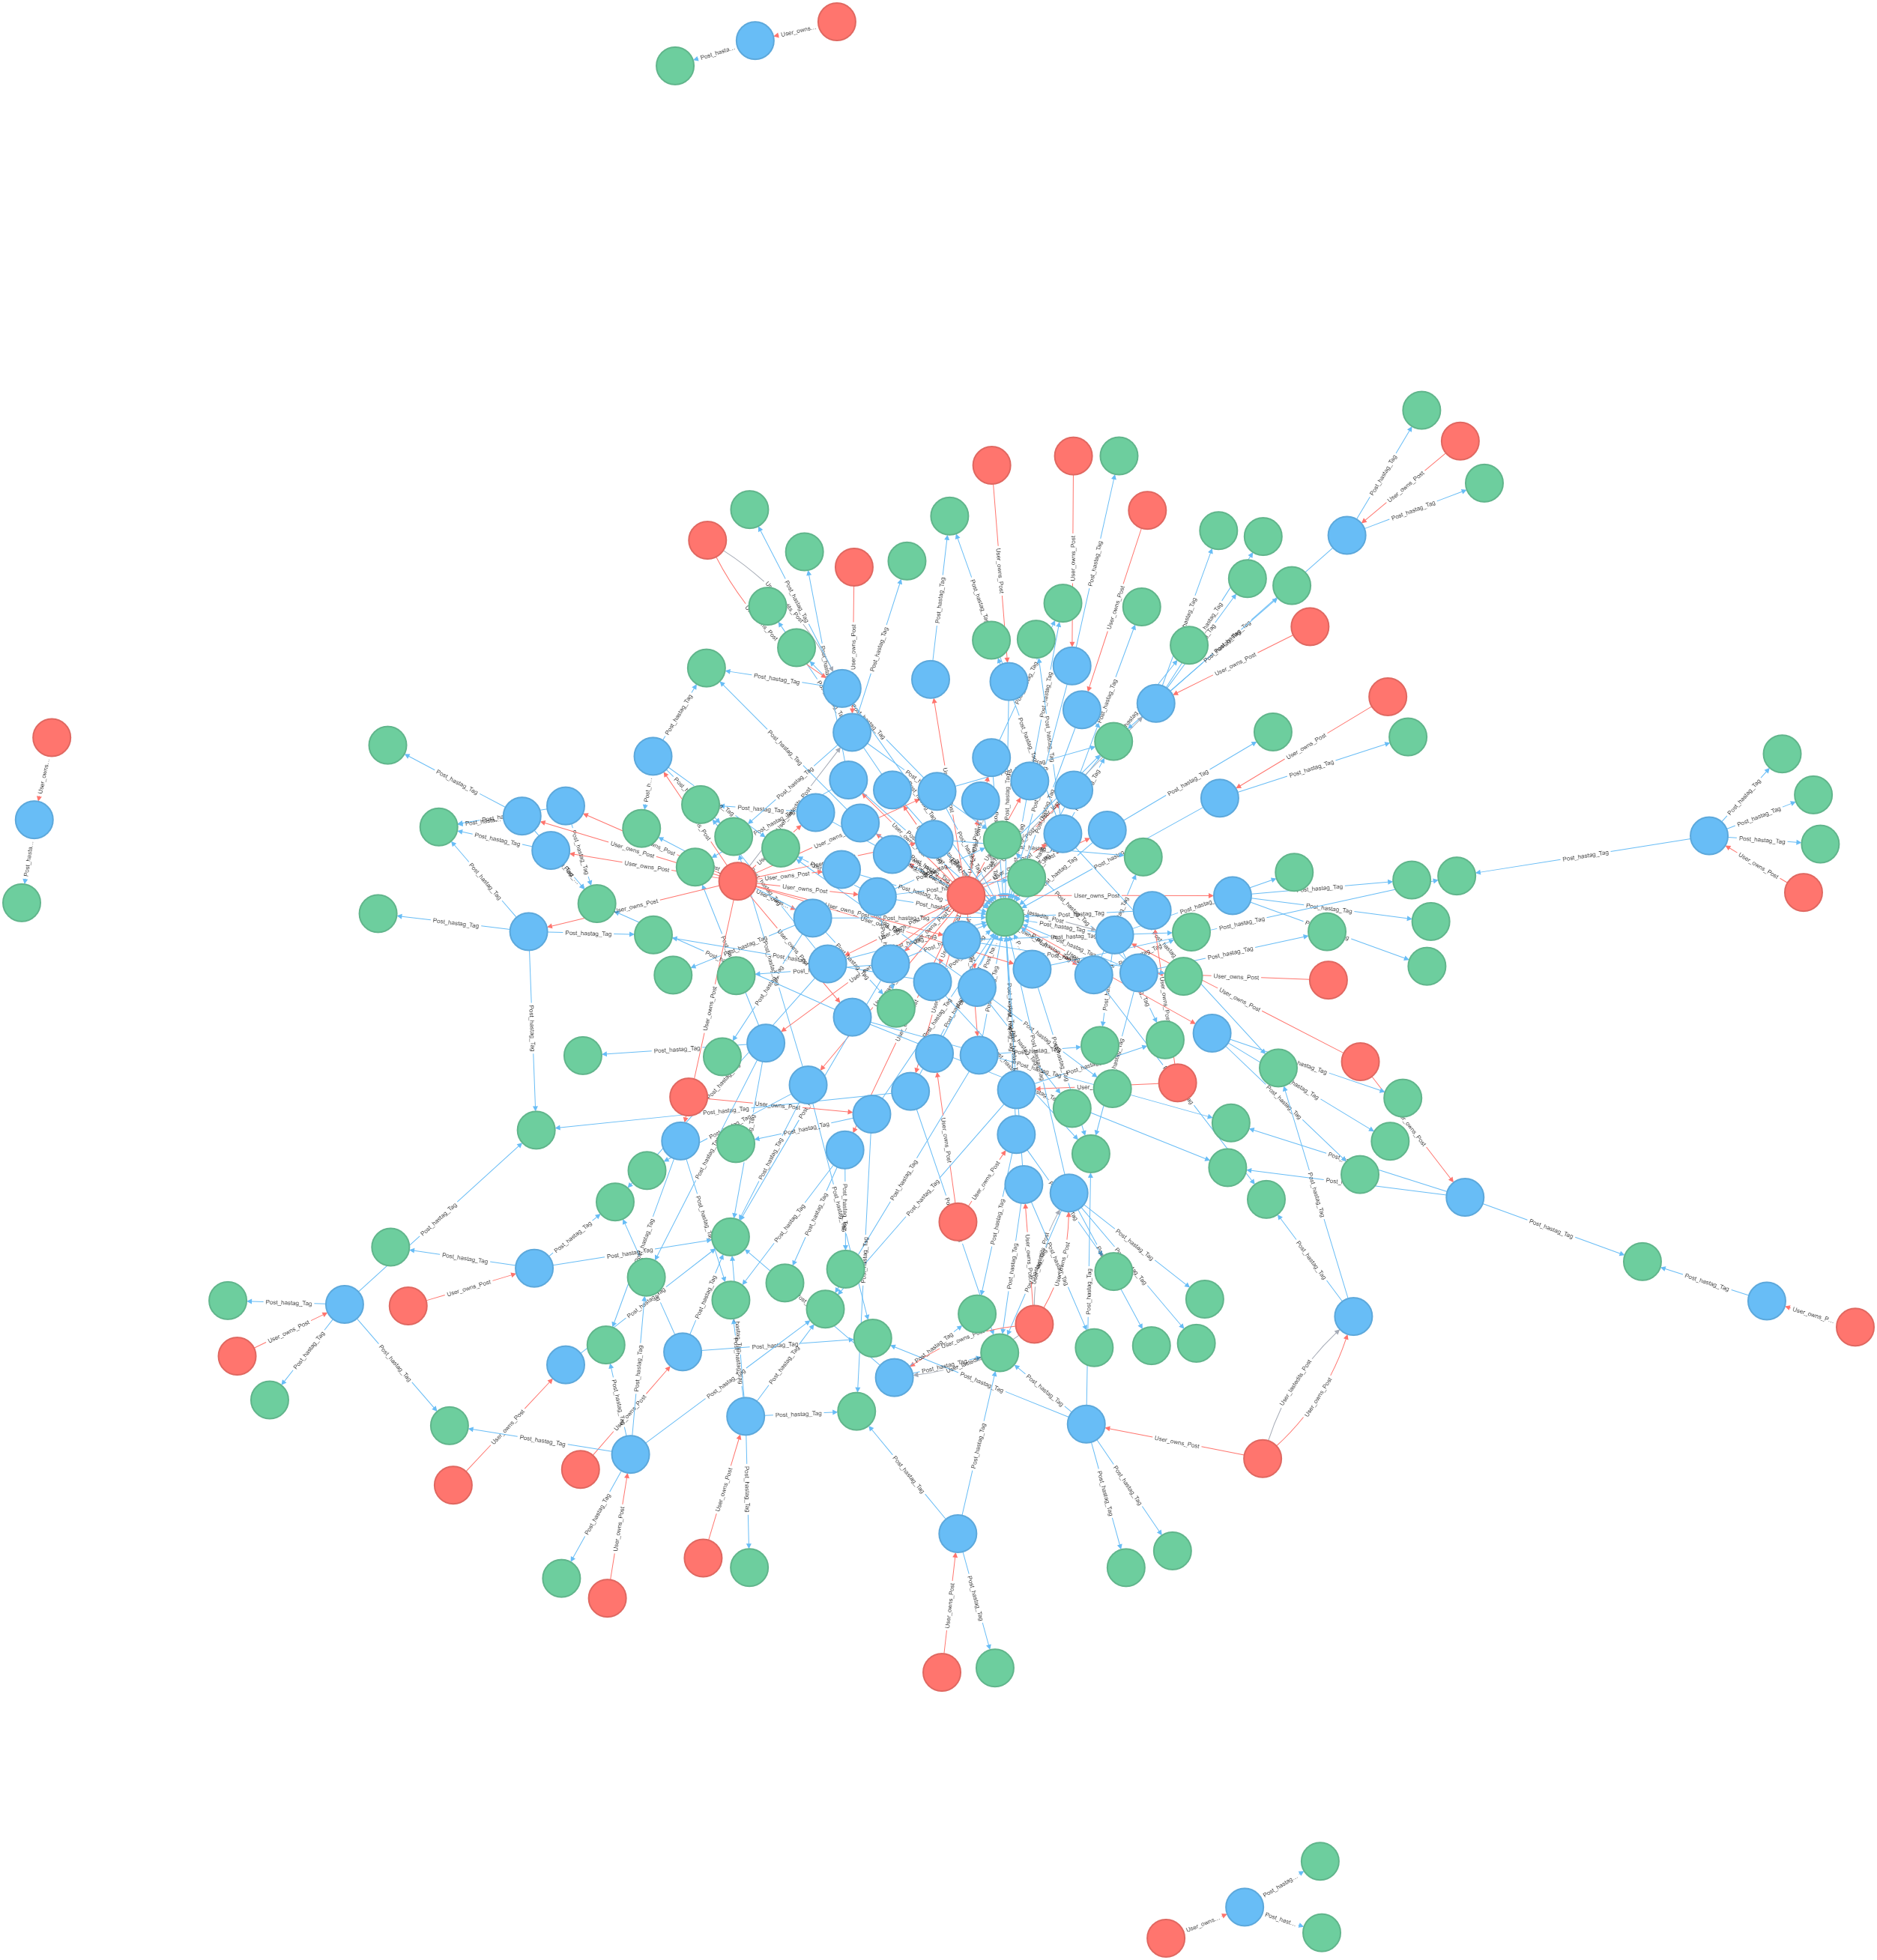
\includegraphics[scale=0.1]{pic/3.png}
\end{figure}

%----------------------------------------------------------------------
\section{Graph OLAP}
%----------------------------------------------------------------------

From the property graph we can ask many interesting questions and queries. Among all kinds of queries, OLAP(Online analytical processing) queries play an important role in business analysis and decision marking. 
 
For example, here are three OLAP queries.
 
Query \#1

Question: 	Does high upvotes of a user indicate a high-quality post?
 
Query: 		Get average post score grouped by user’s upvotes. 

Result:
\begin {center}
 \begin{tabular}{ l l }  
User.UpVotes&AVG(Post.Score)\\0&1.3305406846045096\\1&2.2316044725851976\\2&2.3455564928298624\\3&2.7724084736946435\\4&3.435938918044408\\
 \end{tabular}
 \end {center}

 
 
What we learned:	From the query result we can see that upvotes can be used as a good indicator of a user’s post quality. Suppose we would like to propose suggested posts based on scores. When a post is freshly posted and score of the post has not been well voted been yet, we may use the author’s upvotes as a factor to estimate the quality of his or her post.
 
Query \#2:

Question: 	Following  Query \#1. But this time we want to take a closer look at Query \#1 for different types of questions. If we take upvotes as quality of a user, perhaps quality of a user is shown only in his or her answers, instead of questions. Or is it true that high quality user also asks much better questions?

Query: 		Get average post score grouped by user’s upvotes and post’s post types. 

Result:

\begin {center}
\begin{tabular}{ l l l }
User.Upvotes&Post.PostTypeId&AVG(Post.Score)\\0&1&2.1424667944227734\\1&1&2.2616108846661787\\2&1&2.8346094946401243\\3&1&3.046773386693357\\4&1&3.4642623610482595\\0&2&1.5447668070503877\\1&2&2.2110166471516726\\2&2&2.18900171624714\\3&2&2.7208299711815624\\4&2&3.585763964634491\\
 \end{tabular}
\end {center}


 
What we learned:	From the query result we are suggested that high-quality users not only provide good questions but ask valuable questions as well. However, there is a subtle difference on how upvotes correlate with questions and answers. For instance, a really low upvote level indicates a low-quality answer more than a low-quality question. This is probably because people tend to be more tolerate with a naive question rather than a wrong answer. 
 
Query \#3:

Question: 	In year 2017, which is the weighted average age of users? For instance is ‘python’ more trendy than ‘c’ among young users? 

Query: 		Get average user age grouped by users’ 2017 posts’ tags. 
 
Selected Result:

\begin {center}
\begin{tabular}{ l l  }

TagName&AVG(Age)\\router&19.6\\python&24.1\\internet&26.8\\c&30.2\\programmer&31.4\\software&29.8\\

\end{tabular}
\end {center}


 
What we learned:	We can see the average user age of each tag clearly and easily compare them. For instance, python is generally more popular among younger users. “Router” is a relatively “younger” topic than “internet”. 
 
Query \#4:

Question: 	Follwing Query \#4, let’s look at tendency of topic’s “average popular user age” by years. Is there a tendency of younger age?
 
Query: 		Get average user age grouped by users’ posts’ tags and years. 
 
Selected Result:

\begin {center}
\begin{tabular}{ l l  l}
	
TagName&Year&AVG(Age)\\router&2012&22.1\\router&2017&19.6\\python&2012&27.3\\python&2017&24.1\\internet&2012&27.5\\internet&2017&26.8\\c&2012&30.4\\c&2017&30.2\\programmer&2012&34.2\\programmer&2017&31.4\\software&2012&31.6\\software&2017&29.8\\
	
\end{tabular}
\end {center}
 
What we learned:	Tendency of younger age on IT topics is seen. 
Python is getting faster embraced by younger people compared with C. Similarly we can compare two commercial products’ customer targeting strategy, advitising performance etc. 
 
From the above OLAP query examples we can see that OLAP over property graphs provides an interactive and informative way to analyze property graphs from multiple dimensions and thus helps people find the hidden correlations, aggregated effects, regularities, tendencies and so on. As a matter of fact, OLAP has already played an important role in business analysis and decision making and it is a popular research topic in database area. However most of previous OLAP studies reside in traditional relational data models, whereas studies on OLAP over property graph models are not enough. 


%----------------------------------------------------------------------
\section{Thesis Scope}
%----------------------------------------------------------------------
Graph databases are databases that specialize in storage and processing of property graphs. Unlike traditional relational databases , which adopt traditional way of storing data in form of entity and relationship tables, graph databases store relationships(edges) not as independant tables but directly attached to related entities(nodes)  using data structures such as adjacency lists. 

Many graph database applications have been implemented and commercialized. One of the popular ones is Neo4j. However, current graph databases are not satisfactory in terms of OLAP processing efficiency over large property graphs(with more than millions of nodes and edges). For instance, the above three OLAP queries on a large graph dataset(of roughly 45GB in size) take Neo4j more than 5 hours for Neo4j to process. It is frustrating for users to wait for 2 hours or even more than a day for the result of one OLAP query as this would undermine interactivity which is one of the most best features of OLAP. Therefore we want to accelerate OLAP processing over large property graphs.

\begin{center}
	\begin{tabular}{ | l | l | } 
		\hline 
		Query 	& Time	\\ \hline 
		Query \#1	& \\ \hline
		Query \#2	& \\ \hline
		Query \#3	& \\ \hline
		Query \#4	& \\ \hline
	\end{tabular}
	\end {center}
 

We found that current graph databases like Neo4j process each OLAP query in a naive manner: without using any information of previous queries. In an extreme case, even if we executed a query again and again, execution plan for the query always stays the same and thus execution time does not improve. 

Execution plan of Query \#3 for the first time and execution plan of Query \#3 for the fifth time are the same:
\begin {figure}[H]
\centering
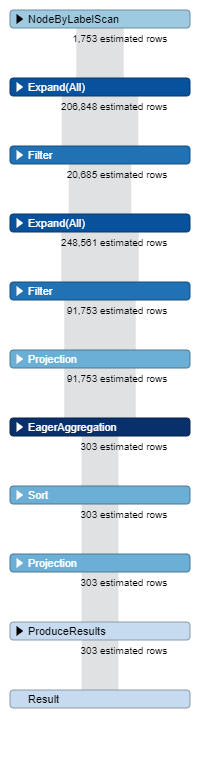
\includegraphics[scale=0.4]{pic/5.png}
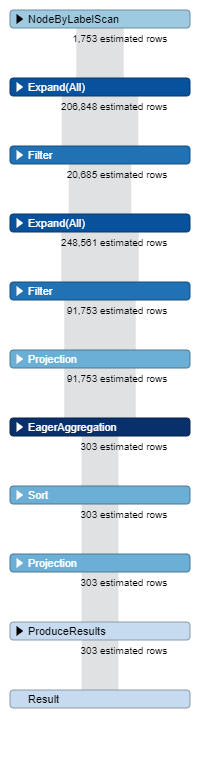
\includegraphics[scale=0.4]{pic/5.png}

\end{figure}

This naive feature of always executing queries regardless of previous queries misses valuable information contained in previous workloads. In reality, most OLAP queries are conducted in a real-time manner. As a result, future queries are unknown before they arrive. However in reality a client’s attention tends to reside in several particular structures and properties (closely related with the topics that the client is interested in). Within a specific time range, it is these “hot” structures that the client tends to repeatedly view in different dimensions. Therefore previous queries can be used as a good reference for understanding which structures and properties the clients are currently interested in. 
 
For instance, suppose a client just executed the exampling four queries, here is what we can learn from these four previous workload:

Structure-wise: (User)-[creates]->(Post) is frequently queried. We can tell that client is interested in how “users creates posts”. Thus it is reasonable to guess that the user is likely to issue OLAP queries involving (User)-[creates]->(Post) in following queries.
 
Property-wise: User.UpVotes, Post.Score, User.Age, Tag.TagName etc. More specifically, <UpVotes, Post.Score> and <User.Age, Tag.TagName> are frequent combinations. Thus it makes sense to guess that these property combinations are likely to appear together in future queries.
 
Intuitively, if we smartly select frequently queried structures and properties based on previous workload and materialize them, they might be covered in future queries and thus be used to accelerate processing. 
 
A good analogy of this is establishment of materialized views in relational databases and processing queries directly on materialized views. In relational databases, we are allowed to build materialized views on structures and attributes that we are interested in. Hopefully when future queries come, we can faster process them using pre-materialized views. Unfortunately, current graph databases do not support similar operations. 
 
Therefore we propose a system that realizes automatic and smart pre computation and materialization based on finished workload, and utilization of materialized result to facilitate faster future query processing. 
 
There are two most important problems that we need to solve: 
 
One key issue is smart selection of “materialized views”. We need to select and pre-compute those that are most beneficial for future queries. 
 
Another key issue is how to optimize a better execution plan for answering a future query efficiently using the precomputed materials.
%----------------------------------------------------------------------
\section{Contribution and Organization}
%----------------------------------------------------------------------
We summurize major contributions of our work is as follows:
\begin{itemize}
\item {We designed an end-to-end system that realizes structure-aware OLAP query processing on graph databases using precomputation based on previous workloads.}

\item We implemented our system on Neo4j.

\item We proposed our algorithm for smart selection of structures and cuboids to be precomputed.
 
\item We suggested different ways for future query processing. We tested their performances and gave explanations on the performance differences.
 
 \end{itemize}

The following contents are organized in this way:
In part 2 we will discuss about related work. We will introduce pre-military knowledge about  OLAP, graph databases, Neo4j; and provide a summary of how existing work solves OLAP queries.
In part 3 we will explain our solution framework and system design in details. 
Part 4 is on experiments. We will talk about experiment design, followed by presentation of experimental results and discussions of results.
Part 5 will talk about opening questions and future work.

